\documentclass[handout, 9pt]{beamer}

%!TEX root = ../notas_de_clase.tex

%preamble

%language
\usepackage[spanish,es-nodecimaldot]{babel}
\usepackage[utf8]{inputenc}
\usepackage{apacite}
\usepackage[absolute,overlay]{textpos}

%packages
\usepackage[Algoritmo]{algorithm}
\usepackage{algorithmicx}
\usepackage[noend]{algpseudocode}
\usepackage{mathtools}
\setlength {\marginparwidth}{2cm}
\usepackage{todonotes}
\usepackage{amsbsy}
\usepackage{amssymb}
\usepackage{amsmath,bm}
\usepackage{dsfont}

\usepackage{xcolor}
\providecommand{\sred}[1]{\textcolor{red}{#1}}
\providecommand{\sblue}[1]{\textcolor{blue}{#1}}
\providecommand{\red}[1]{\textcolor{red}{\text{#1}}}
\providecommand{\blue}[1]{\textcolor{blue}{\text{#1}}}
\providecommand{\redb}[1]{\textcolor{red}{\textbf{#1}}}
\providecommand{\blueb}[1]{\textcolor{blue}{\textbf{#1}}}
\usepackage{graphicx}
\usepackage{fancybox}
\usepackage{booktabs}
\usepackage{caption}
\usepackage{float}
%\usepackage[longend,ruled,algochapter,linesnumbered,lined,boxed,commentsnumbered,spanish]{algorithm2e}
%\usepackage[algo2e]{algorithm2e}
\usepackage{amssymb}
\usepackage{amstext}
\usepackage{bm}
\usepackage{wrapfig}
\usepackage{subcaption} % para_unsupervised_chapter

%formatting

\usepackage[export]{adjustbox}

%caption para figuras
\captionsetup[figure]{width=.8\linewidth, font=small,labelfont={bf},name={Fig.},labelsep=period}
\captionsetup[table]{width=.8\linewidth,font=small,labelfont={bf},name={Tabla},labelsep=period}



\ifx\byn\undefined
    \definecolor{my_blue}{HTML}{C2D5FF}
    \definecolor{my_red}{HTML}{FFC2C2}
    \definecolor{my_yellow}{HTML}{FFFFE0}
\else
    \definecolor{my_blue}{HTML}{FFFFFF}
    \definecolor{my_red}{HTML}{FFFFFF}
    \definecolor{my_yellow}{HTML}{FFFFFF}
\fi


\usepackage[framemethod=TikZ]{mdframed}
\mdfdefinestyle{discusion}{%
    %linecolor=black,
    %outerlinewidth=0pt,
    roundcorner=0pt,
    innertopmargin=5pt,
    innerbottommargin=5pt,
    innerrightmargin=20pt,
    innerleftmargin=20pt,
    backgroundcolor=my_blue}

\colorlet{Green}{green!90}


\mdfdefinestyle{ejemplo}{%
    %linecolor=black,
    %outerlinewidth=0pt,
    roundcorner=0pt,
    innertopmargin=5pt,
    innerbottommargin=5pt,
    innerrightmargin=20pt,
    innerleftmargin=20pt,
    backgroundcolor=my_yellow}


\mdfdefinestyle{pendiente}{%
    style = discusion, 
    backgroundcolor=my_red}


\RequirePackage{url}



%definitions
\def\td{{\text d}}
\def\cN{{\mathcal N}}
\def\cX{{\mathcal X}} 
\def\cC{{\mathcal C}} 
\def\N{{\mathbb N}}
\def\d{{\text d}}
\def\datos{{\mathcal D}}
\def\eye{{\mathbb I}}
\def\ssum{{\scriptstyle\sum}}
\def\bepsilon{{\bm \epsilon}}
\def\tx{\tilde{x}}
\def\tX{\tilde{X}}
\def\thetaMAP{\theta_\text{MAP}}
\newcommand{\gp}{\ensuremath{\mathcal{GP}}}
\newcommand{\pr}{\ensuremath{\mathbb{P}}}
\newcommand{\x}{\ensuremath{\mathbf{x}}}
\newcommand{\z}{\ensuremath{\mathbf{z}}}
\newcommand{\cvector}{\ensuremath{\mathbf{c}}}
\newcommand{\e}{\ensuremath{\mathbf{e}}}
\newcommand{\y}{\ensuremath{\mathbf{y}}}
\newcommand{\bx}{\ensuremath{\textcolor{blue}{X}}}
\newcommand{\by}{\ensuremath{\textcolor{blue}{Y}}}
\newcommand{\rx}{\ensuremath{\textcolor{red}{X_*}}}

\newcommand{\R}{\mathbb{R}}
\newcommand{\norm}[1]{\left\lVert#1\right\rVert}




\DeclareMathOperator*{\argmax}{arg\,max}
\DeclareMathOperator*{\argmin}{arg\,min}
\DeclareMathOperator{\E}{\mathbb{E}}
\DeclareMathOperator{\V}{\mathbb{V}}
\DeclareMathOperator{\KL}{\text{KL}}
\DeclareMathOperator{\MVN}{\text{MVN}}
\newcommand\deq{\stackrel{\mathclap{\normalfont\mbox{\tiny def}}}{=}}
%\newcommand{\E}[1]{\mathbb E \left[#1\right]}
\newcommand{\trace}[1]{\text{Tr} \left[#1\right]}


\usepackage{amsthm}

%-------------------------------------------
% Newtheorem
%-------------------------------------------
\newtheorem{axioma}{\textcolor{red}{Axioma}}
\newtheorem{definicion}{Definición}
\newtheorem*{notacion}{Notación}
\newtheorem{teorema}{Teorema}
\newtheorem{corolario}{Corolario}
\newtheorem{lema}{Lema}
\newtheorem{lemaZ}{\textcolor{red}{Lema}}
\newtheorem{propiedad}{Propiedad:}
\newtheorem{proposicion}{Proposición:}
\newtheorem*{observacion}{Observación}
\newtheorem*{comentario}{Comentario}
\newtheorem*{ejemplo}{Ejemplo}
\newtheorem*{resultado}{Resultado}
\newtheorem*{propuesto}{Ejercicio propuesto}
\newtheorem*{demostracion}{Demostración} % No se usa, usar \begin{proof}\end{proof} que son por default.

%listing paackage para código
\usepackage{listings}
\usepackage{xcolor}
 
\definecolor{codegreen}{rgb}{0,0.6,0}
\definecolor{codegray}{rgb}{0.5,0.5,0.5}
\definecolor{codepurple}{rgb}{0.58,0,0.82}
\definecolor{backcolour}{rgb}{0.95,0.95,0.92}
 
\lstdefinestyle{mystyle}{
    xleftmargin=0.15\textwidth,
    linewidth=0.8\textwidth,
    backgroundcolor=\color{backcolour},   
    commentstyle=\color{codegreen},
    keywordstyle=\color{magenta},
    numberstyle=\tiny\color{codegray},
    stringstyle=\color{codepurple},
    basicstyle=\ttfamily\footnotesize,
    breakatwhitespace=true,         
    breaklines=true,                 
    captionpos=b,                    
    keepspaces=true,                 
    numbers=left,                    
    numbersep=5pt,                  
    showspaces=false,                
    showstringspaces=false,
    showtabs=false,                  
    tabsize=2
}
 
\lstset{style=mystyle}

\numberwithin{equation}{section}

\usetheme{simple}

\title{Clase 3: Regresión lineal (parte 2)}
\subtitle{MDS7104 Aprendizaje de Máquinas}
\date{\today}
\author{Felipe Tobar} 
\titlegraphic{
\begin{figure}[htp] 
    \centering
        
\includegraphics[width=0.15\textwidth]{../img/Uchile.pdf}% 
\end{figure}
}
\institute{Iniciativa de Datos e Inteligencia Artificial\\Universidad de Chile}

\begin{document}
\begin{frame}
  \titlepage
\end{frame}

%Mínimos cuadrados regularizados.
\begin{frame}{Mínimos cuadrados regularizados}

En la clase anterior se vio que el criterio de mínimos cuadrados fallaba cuando los datos presentaban muestras atípicas ya que la penalización cuadrática desplazaba y rotaba el hiperplano regresor.\\~\ \pause

Una forma estándar de corregir parcialmente este problema, es agregar una penalización en la norma del parámetro, logrando que el funcional de costo promueva ajuste a los datos pero también busque parámetros de baja magnitud.\\~\ \pause

De esta forma, el nuevo funcional de costos corresponde a:

\begin{equation*}
	J_\rho = \norm{Y-\tX\theta}_2^2 + \rho\norm{\theta}_p^p,\ p\geq 0,
\end{equation*}

donde $||\cdot||_p$ denota la norma $\ell_p$, es decir, $||\theta||_p=\left(\sum\limits_{j=1}^{M+1}|\theta_j|^p\right)^\frac{1}{p}$ y el parámetro $\rho\geq0$ tiene el rol de balancear la importancia entre ajuste (primer término) y regularidad de la solución (segundo término).
	 
\end{frame}

%¿Por qué penalizar la norma del parámetro?
\begin{frame}{¿Por qué penalizar la norma del parámetro?}

Se podría pensar que el criterio de mínimos cuadrados regularizados (MCR) no puede ser mejor que MC ya que MC se preocupa específicamente de ajustar los datos de forma óptima, mientras que MCR agrega un término que \emph{sesga} la predicción.\\~\ \pause

Este análisis no es del todo correcto ya que: 

\begin{itemize}
	\item MC solo ajusta los datos de entrenamiento y no necesariamente eso produce una buena generalización a datos no observados.\pause
	\item MC presenta una alta varianza cuando el parámetro es de norma alta ya que pequeñas variaciones en la entrada pueden provocar grandes variaciones en la salida.\pause
	\item Por el mismo argumento, si bien MCR agrega un sesgo en la predicción, este es compensado por la disminución de la norma del parámetro $\theta$.\pause
	\item Lo anterior será visto formalmente en la descomposición sesgo-varianza para el caso $p=2$.
\end{itemize}
	
\end{frame}

%Ridge regression o regularización de Tikhonov (p=2).
\begin{frame}{Ridge regression o regularización de Tikhonov ($p=2$)}

Para el caso $p=2$, el funcional tiene la forma

\begin{equation*}
	J_\rho = \norm{Y-\tX\theta}_2^2 + \rho\norm{\theta}_2^2.
	\label{eq:reg_least_squares}
\end{equation*}

Esta regularización es denominada regularización de Tikhonov.\\~\ \pause

El funcional es estrictamente monótono por lo que tiene un único mínimo, el cual puede ser encontrado utilizando la CPO:

\begin{align*}
	&\nabla_\theta J_\rho = 0\nonumber\\
	&\iff -2(Y-\tX\theta)^\top\tX + 2\rho\theta^\top =0\nonumber\\
	&\iff -Y^\top\tX +\theta^\top\tX^\top\tX + \rho\theta^\top= 0\nonumber\\
	&\iff \theta^\top = Y^\top \tX(\tX^\top\tX + \rho\eye)^{-1}\nonumber\\
	&\iff \theta = (\tX^\top\tX+\rho\eye)^{-1}\tX^\top Y.
\end{align*}\pause
	
Se observa que la condición $N>M$ ya no es necesaria, pues la matriz $\tX^\top\tX+\rho\eye$ puede tener determinante tan grande como se quiera simplemente eligiendo un $\rho$ suficientemente grande, solucionando el problema de invertibilidad.	
	
\end{frame}

%Descomposición sesgo-varianza.
\begin{frame}{Descomposición sesgo-varianza}

Una forma de analizar la efectividad de una estimación de un parámetro es mediante la descomposición sesgo-varianza. Se asumirá que las muestras están compuestas de una parte determinista $\tx$ y un ruido aditivo $\epsilon$ (de media nula), es decir:

\begin{equation*}
	y_i = \theta^\top\tx_i + \epsilon_i.
 \end{equation*}\pause
Luego, si $\hat\theta$ es una estimación del parámetro $\theta$, se puede probar que para una nueva observación $(\tx_\star,y_\star)$, el \emph{error cuadrático esperado} asociado a la predicción $\hat y_\star = \hat\theta^\top \tx_\star$ se puede descomponer de la siguiente forma:
 
\begin{equation*}
 	\E{(y_\star - \hat y_\star)^2} = \text{Sesgo}(\hat y_\star)^2 + \text{Varianza}(\hat y_\star) + \sigma^2,\label{eq:expected_sq_loss}
 \end{equation*}

Donde los 3 sumandos de la descomposición corresponden a:\pause
 \begin{itemize}
 	\item $\text{Sesgo}(\hat y_\star) := \E(\hat y_\star) - y_\star$.\pause
 	\item $\text{Varianza}(\hat y_\star) = \E(\E(\hat y_\star)- \hat y_\star)^2$.\pause
 	\item $\sigma^2$ es la varianza de \emph{ruido} $\epsilon$ y no puede ser controlada por la elección de $\hat\theta$.\pause
 \end{itemize}
 
 Es decir, al momento de ajustar un parámetro hay que preocuparse en su sesgo y en su varianza.

\end{frame}

%Sesgo-varianza para ridge regression.
\begin{frame}{Sesgo-varianza para MC y ridge regression}

Para el caso de las estimaciones por mínimos cuadrados y ridge regression se tienen los siguientes resultados:

\begin{teorema}[descomposición sesgo-varianza para MC]
	\begin{align*}
	\text{Sesgo}(\hat f_\star) &= 0\\
	\text{Varianza}(\hat f_\star) &= \sigma^2 \tx_\star^\top (\tX^\top\tX)^{-1}	\tx_\star
\end{align*}
\end{teorema}\pause
	
\begin{teorema}[descomposición sesgo-varianza para ridge regression]
	\begin{align*}
	\text{Sesgo}(\hat f_\star) & = \tx_\star^\top \left((\eye+\rho(\tX^\top\tX)^{-1})^{-1}-\eye\right)\theta\\
	\text{Varianza}(\hat f_\star) &= \sigma^2 \tx_\star^\top (\tX^\top\tX + \rho\eye)^{-1}\tX^\top\tX(\tX^\top\tX+\rho\eye)^{-1}	\tx_\star
\end{align*}

\end{teorema}	\pause
Además, se puede probar que la varianza del estimador de ridge regression es menor a la varianza del estimador de MC.	\\~\ \pause

De esta forma, el parámetro $\rho$ juega el papel de balancear el sesgo y la varianza del estimador.\\~\ 

\textbf{Ejercicio:} Probar los teoremas anteriores. 
	
\end{frame}

%Ejemplo de ridge regression vs. mínimos cuadrados.
\begin{frame}{Ejemplo de ridge regression vs. mínimos cuadrados}

\begin{itemize}
	\item Sean $N=1000$ muestras de un modelo lineal.\pause
	\item Se utilizarán solo $N'=15$ muestras para entrenar el modelo usando MC, y RR con $\rho\in\{40,80\}$.\pause
	\item Se repetirá el proceso 400 veces para analizar como se comportan los estimadores dentro de muestra (con respecto a los datos de entrenamiento) y fuera de muestra (con respecto a los $N-N'$ datos no usados para entrenar).\pause
\end{itemize}
	
\begin{figure}[H]
	\centering
	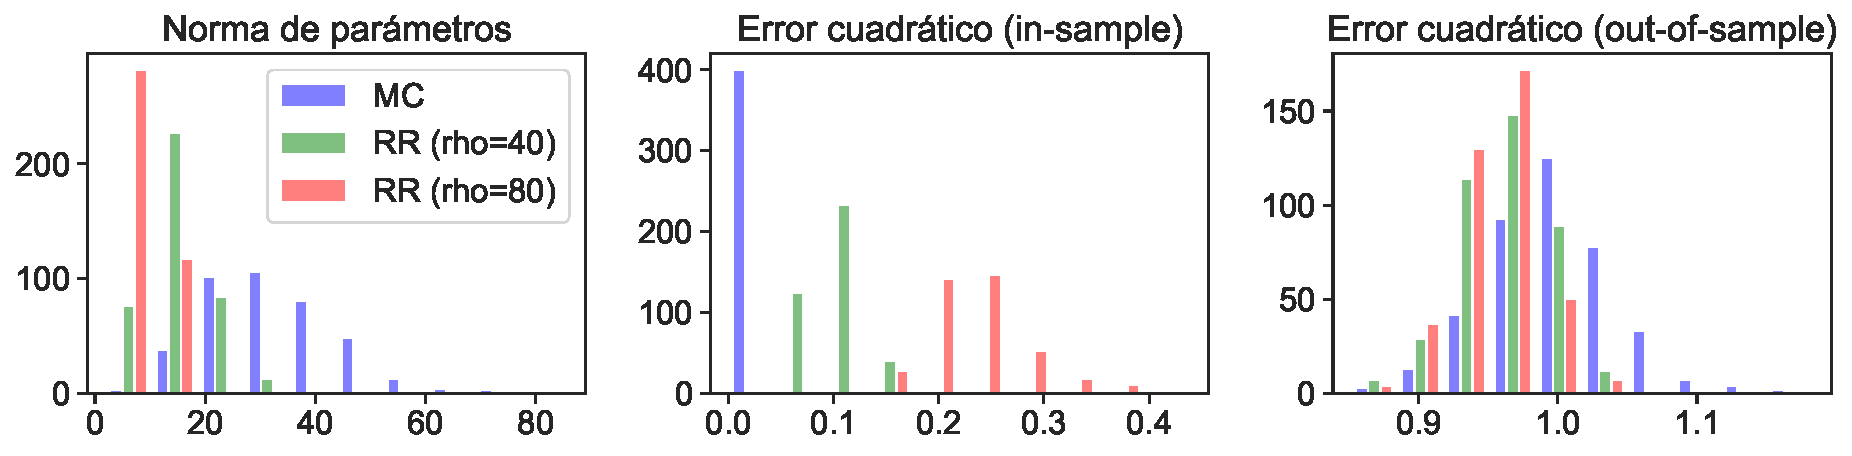
\includegraphics[width=0.8\textwidth]{../img/cap2_bias-variance.pdf}\\
	\label{fig:MCvsRR_Synth}  
\end{figure}\pause

\begin{itemize}
	\item A mayor $\rho$, los parámetros encontrados tienen menor magnitud.\pause
	\item MC se comporta mejor en evaluación dentro de muestra.\pause
	\item RR se comporta mejor en evaluación fuera de muestra.\pause
\end{itemize}

Por lo tanto, se observa que incluir un sesgo en el ajuste del modelo (RR) puede ayudar a generalizar y no sobreajustar cuando se tienen pocos datos. 
		
\end{frame}

%Equivalencia con un problema de optimización con restricción.
\begin{frame}{Regularizar es equivalente a regresión con restricciones}

Si bien el problema de MCR incluye una penalización sobre la norma de $\theta$, el problema también puede ser visto como el problema de MC con la restricción adicional que fija la norma del parámetro. \pause En efecto, podemos expresar dicho problema mediante
\begin{align*}
	\min_\theta  \norm{Y-\tX\theta}_2^2\label{eq:dual_MCR1}
	\quad\text{s.a.} \quad \ ||\theta||_p^p = \tau,
\end{align*}
donde $\tau\geq0$ es una constante fija. \pause El lagrangiano del problema es el siguiente:
\begin{equation*}
	L(\theta,\lambda) = \norm{Y-\tX\theta}_2^2 + \lambda \left(||\theta||_p^p - \tau\right),
\end{equation*}
donde $\lambda$ es el multiplicador de Lagrange asociado al problema. \pause Usando la condición de primer orden se tiene que: 
\begin{align*}
	\frac{\partial L}{\partial \theta} = 0 &\quad\Rightarrow\quad  \frac{\partial }{\partial \theta}\left(\norm{Y-\tX\theta}_2^2 + \lambda ||\theta||_p^p \right) = 0\\
	\frac{\partial L}{\partial \lambda} = 0 &\quad\Rightarrow\quad ||\theta||_p^p = \tau,
\end{align*}\pause
lo cual recupera la forma del problema de MCR. Es decir, se puede interpretar MCR como MC con una restricción sobre la norma.

\end{frame}

\begin{frame}{Curvas de nivel de los regularizadores}
	Con la interpretación anterior, podemos entender distintos regularizadores (distintos $p\geq0$) mediante sus curvas de nivel. La siguiente imagen ilustra las curvas de nivel correspondientes al costo cuadrático (izquierda) y al término de regularización para $p\in\{0.5,1,2\}$. 

\begin{figure}[H]
	\centering
	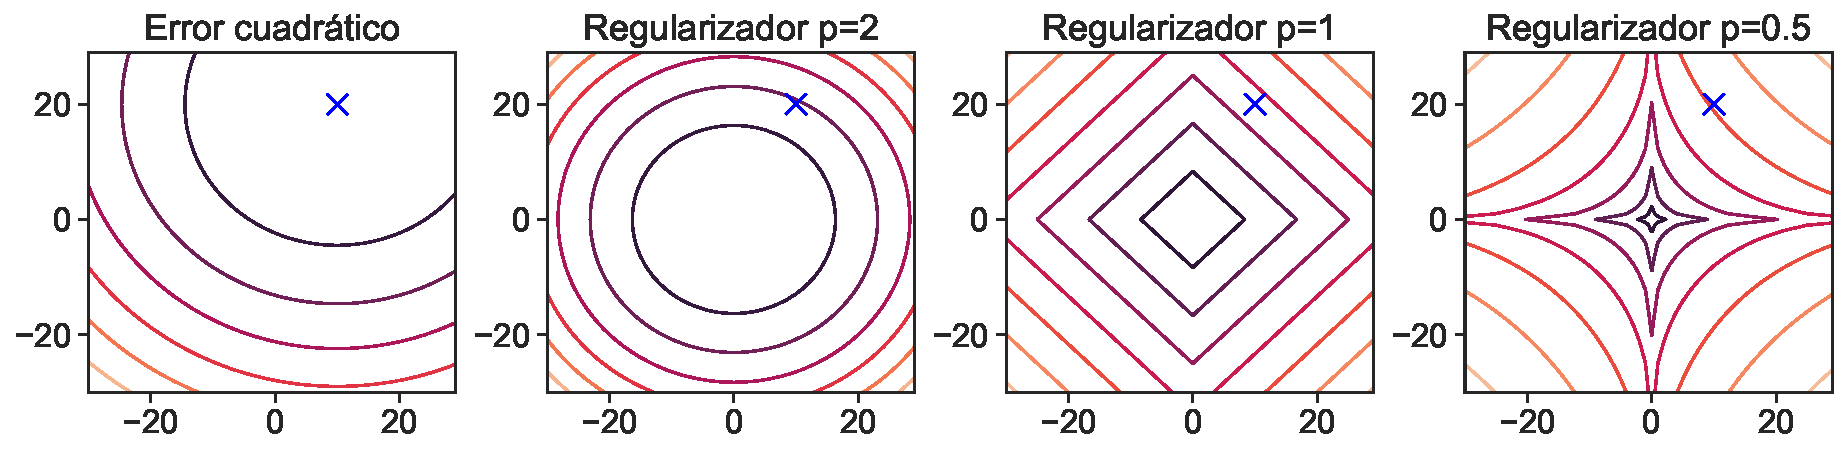
\includegraphics[width=0.8\textwidth]{../img/cap2_regularizadores.pdf}
\end{figure}\pause

Se observa cómo las curvas de nivel atraen el mínimo hacia el origen de distinta forma:

\begin{itemize}
	\item $p=2$ lleva la solución al origen de forma homogénea.\pause
	\item $p\in\{0.5,1\}$ lleva la solución a los bordes, es  decir, privilegiando soluciones ralas.\pause
\end{itemize}

Para $p\leq1$, la forma de la curva de nivel permite que, usualmente, la solución del problema se concentre el las puntas del \emph{diamante}, llevando algunas coordenadas del parámetro $\theta$ directamente a cero. Por esto decimos que $p\leq1$ tiene la propiedad de \emph{selección de variables}.

\end{frame}

\begin{frame}{LASSO y selección de características}

El caso $p=1$ (LASSO), tiene la propiedad de selección de características.\\~\ \pause

Para ilustrar esta propiedad, se utilizará el \emph{Breast Cancer Wisconsin Data Set}\footnote{\url{https://archive.ics.uci.edu/ml/datasets/breast+cancer+wisconsin+(original)}}, el cual tiene $N=569$ muestras y un dimensión de entrada de $M=30$ y se usarán 2/3 de los datos para entrenar y el 1/3 restante para calcular puntajes fuera de muestra. \\

\begin{figure}[H]
	\centering
	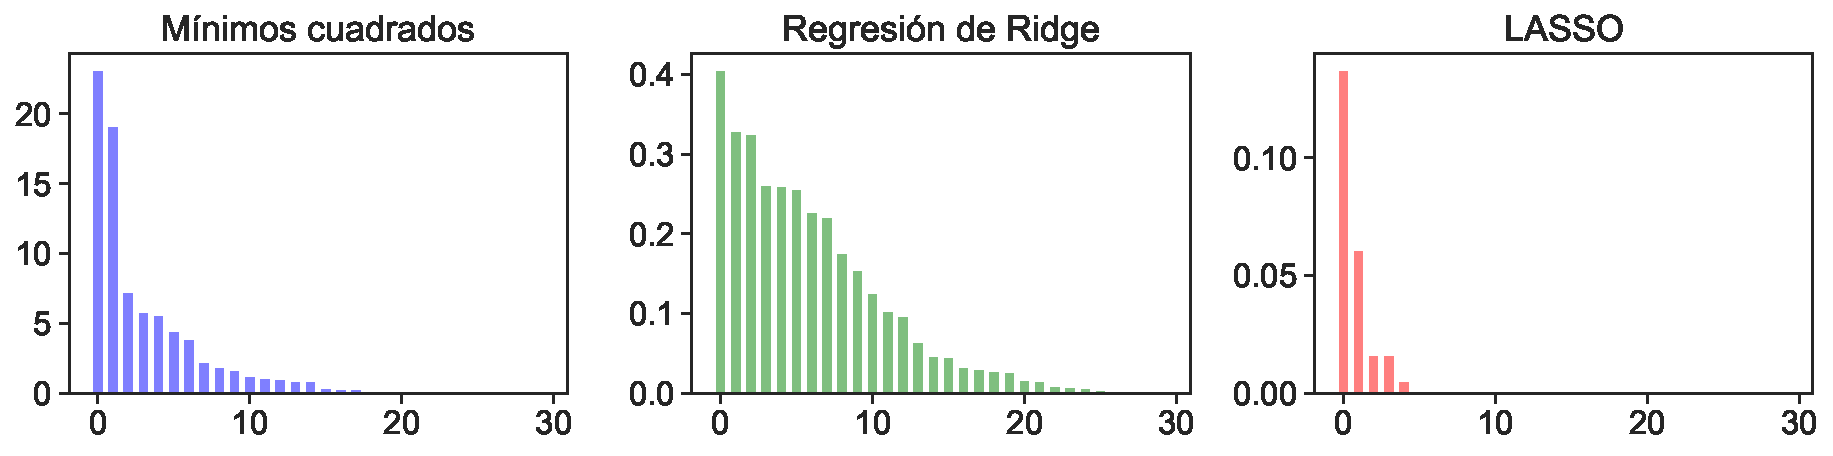
\includegraphics[width=0.8\textwidth]{../img/cap2_OLS_RR_LASSO.pdf}
\end{figure} \pause

Se observa la disminución en la norma de $\theta$ al usar MCR, así como también la selección de características realizada por LASSO.\pause

\begin{table}[h]
\centering
\footnotesize
	\begin{tabular}{ r|c|c } 
		 & in-sample & out-of-sample \\
		\hline
		MC & \textbf{0.7896} & 0.6911 \\ 
		RR & 0.6905 & 0.6903 \\ 
		LASSO & 0.7452 & \textbf{0.7242}
	\end{tabular}
\end{table}

 Notar que LASSO tiene el mejor puntaje fuera de muestra.

\end{frame}

\begin{frame}{Elastic net y consideraciones generales}

Para concluir esta sección, es importante tener en cuenta que:

\begin{itemize}
	\item Una posible variación de MCR consiste en utilizar la regularización LASSO y ridge al mismo tiempo, resultando en lo que se denomina \emph{elastic net regularization}, cuyo funcional de costo es

\begin{equation*}
	J_\rho = \norm{Y-\tX\theta}_2^2 + \lambda_1\norm{\theta}_2^2 + \lambda_2\norm{\theta}_1.
\end{equation*} \pause

	\item Como se vio en la descomposición sesgo-varianza, el \emph{hiperparámetro} $\rho$ determina el balance entre regularización (cuán  sesgado) y ajuste (cuán bien replica  los datos de entrenamiento). En la práctica, para elegir este hiperparámetro se puede evaluar el desempeño fuera de muestra para distintos valores de $\rho$ con la finalidad de elegir un valor apropiado. Una manera de realizar la evaluación de desempeño para diferentes $\rho$ será vista al estudiar la \emph{validación cruzada}.
\end{itemize}

	
\end{frame}

\end{document}
